%%%%%%%%%%%%%%%%%%%%%%%%%%%%%%%%%%%%%%%%%%%%%
\section{Initial data far from equilibrium}
\label{Sec:FarFromEq}
%%%%%%%%%%%%%%%%%%%%%%%%%%%%%%%%%%%%%%%%%%%%%

In this section we consider the gas cloud~(\ref{Eq:Pulse}), which is concentrated about one orbital phase and is far from any steady state, and we analyze how its evolution changes when its mass is increased. We start with the simulations and with a parameter $\mu$ which compares the attraction of the cloud with the spread of its orbital frequencies. Next, we show that the cloud mixes when $\mu$ is small and collapses into a self-bound clump which does not mix when $\mu$ exceeds a critical value, and we analyze the dependence of this value on the widths of the cloud and on the external potential. Finally, we describe the state of the gas at late times.


\subsection{Simulations and the parameter $\mu$}
\label{SubSec:FarRuns}

The reference family of simulations consists of the cloud~(\ref{Eq:Pulse}) with $\sigma_Q = \sigma_J = 0.1$ and $L_0 = 2$ in the isochrone potential, with the masses $M_{gas}/M = 10^{-3}$, $0.01$, $0.015$, $0.02$, $0.025$, $0.03$, $0.04$, $0.05$, $0.07$, $0.1$ and $0.3$, together with a simulation without self-gravity. In order to analyze the dependence on the shape of the cloud, we vary its width in angle, $\sigma_Q = 0.2$ and $0.4$ with $M_{gas}/M = 0.01$, $0.02$, $0.04$ and $0.08$, and its width in action, $\sigma_J = 0.05$ with $M_{gas}/M = 0.005$, $0.01$ and $0.02$ and $\sigma_J = 0.2$ with $M_{gas}/M = 0.02$, $0.04$ and $0.08$. Finally, we consider the cloud with $\sigma_Q = \sigma_J = 0.1$ in the Kepler potential, with $M_{gas}/M = 0.01$, $0.02$, $0.04$ and $0.08$. This is the external potential of the nonlinear phase mixing result of Ref.~\cite{sCjL26}, although the reduced model and the support of the DF, which extends to the circular orbit, differ from the assumptions made there. The simulations use the lattice~(\ref{Eq:Lattice}) with $N_J\times N_Q = 400\times 25$, except for $\sigma_Q = 0.2$ ($N_Q = 50$) and $\sigma_J = 0.2$ ($N_J = 800$), and the time step $\Delta t = 0.05$, and they extend to $t = 10^4$ ($2\times 10^4$ for $\sigma_J = 0.05$). In order to test the convergence, we have repeated the simulations of the reference family with $M_{gas}/M = 0.01$, $0.02$ and $0.1$ with $N_Q = 100$, and the one with $M_{gas}/M = 0.01$ with $N_J = 800$. In all the simulations the gas particles remain bound, and the observables are computed with the action-angle variables of the instantaneous potential and the weight function $B = 1$, see sections~\ref{SubSec:Observables} and~\ref{SubSec:PIC}.

In the absence of self-gravity the cloud mixes on a time scale which is set by the spread of its orbital frequencies. We characterize this spread by the interval $[\underline{J},\overline{J}]$ in which the factor $J^2\exp(-J^2/\sigma_J^2)$ of the DF~(\ref{Eq:Pulse}) exceeds one percent of its maximum, by its width $\Delta J := \overline{J} - \underline{J}$, and by the width $\Delta\Omega := \Omega(\underline{J}) - \Omega(\overline{J})$ of the corresponding frequency band of the external potential. After the time
\begin{equation}
\tau_1 := \frac{2\pi}{\Delta\Omega}
\label{Eq:tau1}
\end{equation}
the orbits at the two ends of this interval have drifted apart by one revolution, such that the first harmonic of the cloud has been spread over the orbit. For $\sigma_Q = \sigma_J = 0.1$ in the isochrone potential one has $\Delta J = 0.270$, $[\Omega(\overline{J}),\Omega(\underline{J})] = [0.0513,0.0705]$ and $\tau_1 = 327$, for $\sigma_J = 0.05$ and $0.2$ one has $\tau_1 = 589$ and $198$, respectively, and in the Kepler potential $\tau_1 = 161$. Hence, the simulations extend over at least $30$ units of $\tau_1$.

The self-gravity of the cloud opposes the mixing, since it attracts the gas particles towards the center of the cloud. In order to compare both effects, consider a gas particle with action variable $J$ and let $\vartheta$ denote its angle variable relative to the one of the center of the cloud. In the absence of self-gravity, $\vartheta$ drifts with a velocity which varies by $\Delta\Omega$ across the support of the cloud. Approximating the derivative of the frequency by the constant $|\Omega'| = \Delta\Omega/\Delta J$ and the potential of the cloud by a well of the form $A\cos\vartheta$, one obtains a pendulum of the form~(\ref{Eq:Pendulum}), with $2\varepsilon|\phi_1|$ replaced by $A$, whose bounce frequency and separatrix half-width are $\omega_b = (|\Omega'| A)^{1/2}$ and $\Delta J_s = 2\omega_b/|\Omega'|$, see Eq.~(\ref{Eq:Separatrix}). This suggests the parameter
\begin{equation}
\mu := \frac{\omega_b}{\Delta\Omega} = \left( \frac{A}{\Delta\Omega\,\Delta J} \right)^{1/2},
\label{Eq:muDef}
\end{equation}
which compares the bounce frequency in the potential well of the cloud with the spread of its orbital frequencies. In terms of it, the bounce period is $2\pi/\omega_b = \tau_1/\mu$ and the separatrix half-width is $\Delta J_s = 2\mu\,\Delta J$, such that the separatrix covers the support of the cloud when $\mu > 1/4$. This picture is only a heuristic one, since the potential of the cloud is not a single harmonic and the cloud is not small compared with the separatrix. We measure $A$ as half of the largest variation of $\Phi_{gas}(t,r)$ at fixed $r$ during the first radial period $0\leq t\leq 2\pi/\Omega(\overline{J})$, maximized over $3\leq r\leq 15$. For small masses $A$ is proportional to the mass of the gas: in the reference family $A = 4.9\times 10^{-5}$ and $4.9\times 10^{-4}$ for $M_{gas}/M = 10^{-3}$ and $10^{-2}$, such that $\mu$ grows like $(M_{gas}/M)^{1/2}$. For these two masses $\mu = 0.10$ and $0.31$, and for $M_{gas}/M = 0.1$ and $0.3$ one has $\mu = 0.89$ and $1.16$.


\subsection{Mixing and self-bound clump}
\label{SubSec:FarRegimes}

\begin{figure}[htp]
\centerline{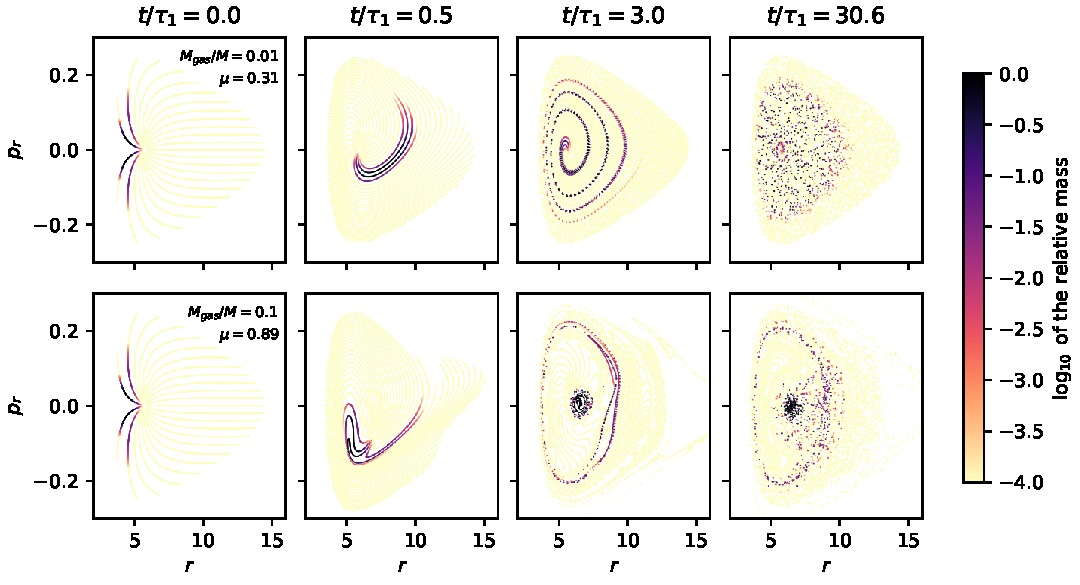
\includegraphics[width=\textwidth]{figuras/bulto_fase.pdf}}
\caption{The computational particles in the $(r,p_r)$-plane at four different times for the cloud~(\ref{Eq:Pulse}) with $\sigma_Q = \sigma_J = 0.1$ in the isochrone potential, for $M_{gas}/M = 0.01$ (upper panels) and $M_{gas}/M = 0.1$ (lower panels). The color indicates the mass of each particle relative to the largest one. For $M_{gas}/M = 0.01$ the cloud mixes, whereas for $M_{gas}/M = 0.1$ it forms a clump which persists until the end of the simulation.}
\label{Fig:CloudPhase}
\end{figure}

Figure~\ref{Fig:CloudPhase} shows the computational particles in the $(r,p_r)$-plane for two clouds of the reference family. For $M_{gas}/M = 0.01$ ($\mu = 0.31$) the evolution resembles the mixing without self-gravity of Fig.~\ref{Fig:Pulse}: the cloud is sheared into a spiral which winds up around the circular orbit, and at $t = 30\tau_1$ the gas fills the region of phase space which is covered by its orbits, without any visible concentration. For $M_{gas}/M = 0.1$ ($\mu = 0.89$), in contrast, a part of the cloud contracts within the first radial periods into a compact clump, which does not mix: at $t = 30\tau_1$ it is still present, and the rest of the gas is mixed around it. The center of the clump oscillates radially about the circular orbit. Defining the clump by the particles whose action variable is smaller than $0.05$ at $t = 10^4$, we find that for $t\geq 15\tau_1$ its center moves between $r = 4.8$ and $r = 6.5$, with the frequency $0.075$, while the root mean square distance of its particles from the center is $0.3$. This frequency is close to the frequency $\Omega(0) = 0.0711$ of the circular orbit in the external potential.

\begin{figure}[htp]
\centerline{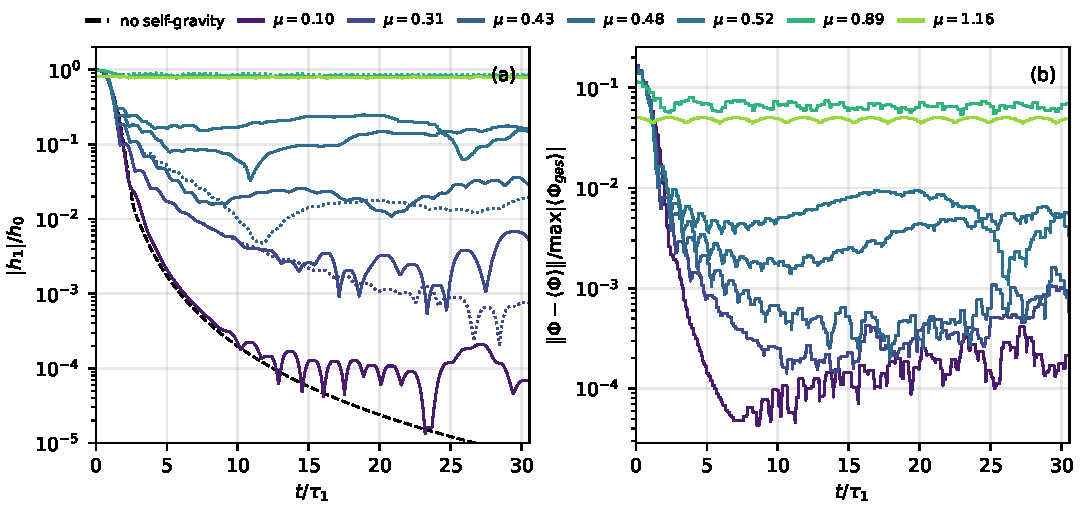
\includegraphics[width=\textwidth]{figuras/bulto_series.pdf}}
\caption{Evolution of the cloud~(\ref{Eq:Pulse}) with $\sigma_Q = \sigma_J = 0.1$ in the isochrone potential for different masses, labeled by the value of $\mu$. (a) Envelope of $|h_1|/h_0$ (largest value in a moving window of width $100$), computed with the action-angle variables of the instantaneous potential, for $N_J\times N_Q = 400\times 25$ (solid lines) and $400\times 100$ (dotted lines). (b) Deviation of the potential from its average over the second half of the simulation, measured with the norm~(\ref{Eq:deltaPhiNorm}) over $3\leq r\leq 15$ in units of the largest value of $|\langle\Phi_{gas}\rangle|$ (envelope as in (a)).}
\label{Fig:CloudSeries}
\end{figure}

The function $|h_1(t)|/h_0$ and the oscillation of the potential are shown in Fig.~\ref{Fig:CloudSeries} for the reference family. Without self-gravity, $|h_1|$ decays like $t^{-3}$ (a fit of the envelope over $10\leq t/\tau_1\leq 30$ gives the exponent $-3.03$), which is the analogue of the tail~(\ref{Eq:Tail}) for the endpoint $J = 0$ of the support, at which $\hat{F}_1$ vanishes like $J^2$. With self-gravity the decay slows down, and the level which is reached at late times increases with $\mu$. Averaged over $10\leq t/\tau_1\leq 20$, $|h_1|/h_0$ is $1.1\times 10^{-4}$, $2.4\times 10^{-3}$ and $1.2\times 10^{-2}$ for $\mu = 0.10$, $0.31$ and $0.43$ (the last two values for $N_Q = 100$), compared to $7.0\times 10^{-5}$ without self-gravity, and it lies between $0.09$ and $0.85$ for $\mu\geq 0.48$. The potential behaves in the same way. In the second half of the simulations its deviation from the average $\langle\Phi\rangle$ over this interval, measured as in Fig.~\ref{Fig:CloudSeries}(b), lies between $5\times 10^{-5}$ and $4\times 10^{-4}$ for $\mu\leq 0.43$, whereas it lies between $3\times 10^{-3}$ and $5\times 10^{-2}$ for $\mu\geq 0.48$. Hence, for $\mu\leq 0.43$ the potential becomes stationary, whereas for $\mu\geq 0.48$ it keeps oscillating with the clump.


\subsection{The transition}
\label{SubSec:FarTransition}

\begin{figure}[htp]
\centerline{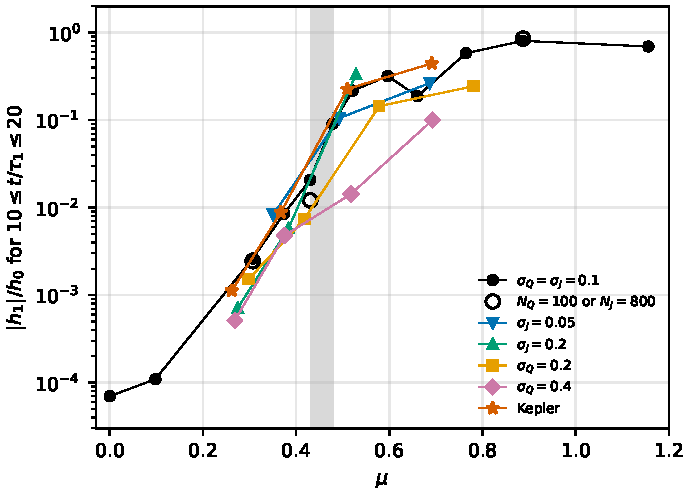
\includegraphics[width=0.6\textwidth]{figuras/bulto_transicion.pdf}}
\caption{Mean value of $|h_1|/h_0$ over the interval $10\leq t/\tau_1\leq 20$ as a function of the parameter~(\ref{Eq:muDef}), for all the simulations of the cloud~(\ref{Eq:Pulse}). The families differ in the widths $\sigma_Q$ and $\sigma_J$ of the cloud (equal to $0.1$ unless otherwise stated) and in the external potential (isochrone unless otherwise stated). The open circles refer to the simulations of the reference family with $N_Q = 100$ or $N_J = 800$. The shaded band indicates the interval $0.43\leq\mu\leq 0.48$.}
\label{Fig:CloudTransition}
\end{figure}

Figure~\ref{Fig:CloudTransition} shows the mean value of $|h_1|/h_0$ over the interval $10\leq t/\tau_1\leq 20$ as a function of $\mu$ for all the simulations. In each family, $|h_1|/h_0$ grows by one to two orders of magnitude within a narrow interval of $\mu$. With the exception of the family with $\sigma_Q = 0.4$, the location of this interval is the same for all the families: all the simulations with $\mu\leq 0.43$ have $|h_1|/h_0\leq 2.1\times 10^{-2}$, and all those with $\mu\geq 0.48$ have $|h_1|/h_0\geq 0.09$. Table~\ref{Tab:Critical} lists, for each family, the largest value of $\mu$ for which the cloud mixes and the smallest one for which it forms a clump. The intervals which are delimited by these values have the common part $0.43\leq\mu\leq 0.48$ for the five families with $\sigma_Q\leq 0.2$, whereas for $\sigma_Q = 0.4$ the transition lies between $\mu = 0.52$ and $\mu = 0.69$. Therefore, for clouds which are compact in angle the critical value $\mu_c$ of the parameter~(\ref{Eq:muDef}) lies between $0.43$ and $0.48$, independently of the width of the cloud in action and of the external potential, whereas a cloud which is wide in angle requires a larger value of $\mu$ in order to form a clump. The critical value is of the order of the estimate $\mu = 1/4$ of the pendulum picture, but about twice as large, which is not surprising, since $A$ is only a proxy for the amplitude of the potential of the cloud along the orbits. Hence, $\mu$ captures the competition between self-gravity and shear for compact clouds, but not the complete dependence on the shape of the cloud. \EJ{A theory of $\mu_c$, including its dependence on $\sigma_Q$, is still missing.}

\begin{table}[htp]
\begin{center}
\begin{tabular}{ll|cc|cc}
\hline\hline
 & & \multicolumn{2}{c|}{mixing} & \multicolumn{2}{c}{clump} \\
potential & widths & $\mu$ & $|h_1|/h_0$ & $\mu$ & $|h_1|/h_0$ \\
\hline
isochrone & $\sigma_Q = \sigma_J = 0.1$ & $0.43$ & $1.2\times 10^{-2}$ & $0.48$ & $0.091$ \\
 & $\sigma_J = 0.05$ & $0.35$ & $8.3\times 10^{-3}$ & $0.49$ & $0.105$ \\
 & $\sigma_J = 0.2$ & $0.38$ & $5.8\times 10^{-3}$ & $0.53$ & $0.33$ \\
 & $\sigma_Q = 0.2$ & $0.42$ & $7.4\times 10^{-3}$ & $0.58$ & $0.14$ \\
 & $\sigma_Q = 0.4$ & $0.52$ & $1.4\times 10^{-2}$ & $0.69$ & $0.10$ \\
Kepler & $\sigma_Q = \sigma_J = 0.1$ & $0.37$ & $8.8\times 10^{-3}$ & $0.51$ & $0.23$ \\
\hline\hline
\end{tabular}
\end{center}
\caption{Bracketing of the transition: for each family, the largest value of $\mu$ for which the cloud mixes and the smallest one for which it forms a clump, together with the mean value of $|h_1|/h_0$ over $10\leq t/\tau_1\leq 20$. In the family with $\sigma_J = 0.05$ ($\sigma_Q = 0.2$, $0.4$) the remaining width is $\sigma_Q = 0.1$ ($\sigma_J = 0.1$). For $\mu = 0.43$ the value refers to $N_Q = 100$; for $N_Q = 25$ it is $2.1\times 10^{-2}$.}
\label{Tab:Critical}
\end{table}

Away from the transition the results do not depend on the resolution. For $\mu = 0.31$ we obtain $|h_1|/h_0 = 2.62\times 10^{-3}$ with $N_J\times N_Q = 400\times 25$ and $2.44\times 10^{-3}$ with both $400\times 100$ and $800\times 25$, and for $\mu = 0.89$ we obtain $0.80$ with $400\times 25$ and $0.85$ with $400\times 100$. Close to the transition, in contrast, the result depends on the number of particles: for $\mu = 0.43$ it is $2.1\times 10^{-2}$ with $400\times 25$ and $1.2\times 10^{-2}$ with $400\times 100$. This is to be expected, since near the threshold the outcome is sensitive to small perturbations, such as those which are due to the discreteness of the particles. However, both simulations lie on the same side of the transition.

In the Kepler potential the clouds with $M_{gas}/M = 0.01$ and $0.02$ ($\mu = 0.26$ and $0.37$) mix, which is the behavior described by Ref.~\cite{sCjL26} for small data, whereas those with $M_{gas}/M = 0.04$ and $0.08$ ($\mu = 0.51$ and $0.69$) form a clump. Since $\mu$ grows with the mass, for a cloud of a given shape the mixing fails above a critical mass, which lies between $M_{gas}/M = 0.02$ and $0.04$ in this case. Hence, in the reduced model, the phase mixing of such a cloud requires its mass to be small.


\subsection{The state at late times}
\label{SubSec:FarLate}

Below the transition, the mixing continues after the decay of Fig.~\ref{Fig:CloudSeries}(a) has slowed down. In the simulations of the reference family with $\mu = 0.31$ and $N_Q = 100$ or $N_J = 800$, $|h_1|/h_0$ decreases from $2.4\times 10^{-3}$ for $10\leq t/\tau_1\leq 20$ to $7.5\times 10^{-4}$ and $8.6\times 10^{-4}$ for $t/\tau_1\geq 20$, respectively. With the default lattice, in contrast, it remains at $2.8\times 10^{-3}$, which is due to the fluctuations generated by the discreteness of the particles (see section~\ref{SubSec:ValAA}). Hence, the self-gravity of the cloud slows down the mixing, as for the perturbations of a steady state of section~\ref{SubSec:FixedLDamped}, but it does not stop it. A quantitative analysis of this late decay requires larger numbers of particles than those used here. \EJ{To be determined with $N\geq 10^5$ particles: the decay law of $|h_1|$ below the transition.}

Above the transition the clump persists until the end of the simulations. For $0.76\leq\mu\leq 1.16$ the amplitude of the radial oscillation of its center decreases by at most $25$ percent between the intervals $3\leq t/\tau_1\leq 10$ and $20\leq t/\tau_1\leq 30$, and not at all for $\mu = 1.16$, such that within the time span of our simulations the oscillation does not die out. The value of $|h_1|$ is not a monotonic function of $\mu$ above the transition: for $\mu = 0.52$, $0.60$, $0.66$, $0.76$, $0.89$ and $1.16$ it is $0.22$, $0.32$, $0.19$, $0.58$, $0.80$ and $0.69$, respectively. This reflects the amplitude of the oscillation of the clump, which determines how strongly the gas is concentrated in angle. For $\mu = 0.66$, for instance, the center of the clump moves by $\pm 0.16$ about its mean radius, which is less than the size $0.32$ of the clump, whereas for $\mu = 0.89$ it moves by $\pm 0.9$. The mass of the clump cannot be determined in a unique way by means of a cut in the action variable: for $\mu = 0.89$ the particles with $J < 0.03$, $0.05$ and $0.08$ at $t = 10^4$ carry $58$, $75$ and $83$ percent of the mass of the gas, and below the transition such cuts also select part of the mixed gas (for $\mu = 0.31$, $21$ percent of the mass has $J < 0.05$). For this purpose a dynamical criterion would be required, which identifies the particles that are bound to the clump. \EJ{To be done: a dynamical criterion for the mass of the clump.}

The state above the transition, which consists of a compact clump whose oscillation persists and of mixed gas around it, resembles the core-halo states which are formed by collisionless relaxation in systems with long-range interactions~\cite{yLrPfRtTfB14}. In the scenario described in that reference, the particles which are in parametric resonance with the oscillation of the core escape to the halo, and this damps the oscillation until a quasi-stationary state is reached. In our simulations the oscillation of the clump is damped only slowly, if at all, over $30$ units of $\tau_1$.
